\chapter{调度}\label{ch07}

任何操作系统都可能需要运行比处理器数量更多的进程,因此需要一个计划来在进程之间共享处理器。理想状态下这种共享对用户进程来说应该是透明的。一个通用的解决方案是通过在多个进程间\emph{多路复用(multiplex)}硬件处理器来给每个进程提供虚拟的处理器。这一章将解释xv6如何实现这种复用。

\section{多路复用}
xv6在两种情况下会把CPU从一个进程切换到另一个进程。
一个是,xv6的\texttt{sleep}和\texttt{wakeup}机制会在进程等待设备或管道I/O完成、等待子进程退出、在\texttt{sleep}系统调用中等待时切换进程。
另一个是,xv6会周期性的强制切换以应对长时间计算无需睡眠的进程。
这种多路复用创造出了每个进程都有单独的CPU的假象,类似于xv6使用内存分配器和硬件分页表来创造每个进程都有单独的内存的假象。

实现多路复用也面临一些挑战。
第一,如何从一个进程切换到另一个?
尽管上下文切换的思路很简单,但实现是xv6中最不透明的部分之一。
第二,如何以一种对用户透明的方式强制切换进程?
xv6使用了标准的计数,也就是用硬件时钟的中断来驱动上下文的切换。
第三,所有的CPU在一个共享的进程集合中切换,因此需要一种加锁的方案来避免竞争。
第四,一个进程的内存和其他资源必须在进程退出时释放,但这个过程并不能完全由进程自身来实现,例如它不能在使用中释放它自己的内核栈。
第五,多核机器的每个核心都必须记住它正在执行哪个进程,这样系统调用才能影响到正确的进程的内核状态。
最后,\texttt{sleep}和\texttt{wakeup}允许一个进程放弃CPU并等待被另一个进程或中断唤醒。
需要小心避免导致唤醒通知丢失的竞争。
xv6尝试尽可能简单地解决这些问题,但最终的代码仍然很棘手。

\section{代码:上下文切换}
\autoref{f7-1}概述了从一个进程切换到另一个进程的步骤:一个用户到内核的切换(通过系统调用或者中断)到达旧进程的内核线程,一个上下文切换到达当前CPU的调度器线程,一个上下文切换到新进程的内核线程,一个自陷返回到用户级的进程。
xv6的每个CPU的调度器有一个专用的线程(有自己的寄存器和栈),因为让调度器在旧进程的内核栈上执行是不安全的:其他的核心可能会唤醒这个进程然后运行它,然后在两个核心上同时使用同一个栈将会导致灾难。
在这一节中我们将研究在内核线程和调度器线程之间切换的机制。

\begin{figure}[htbp]
    \centering
    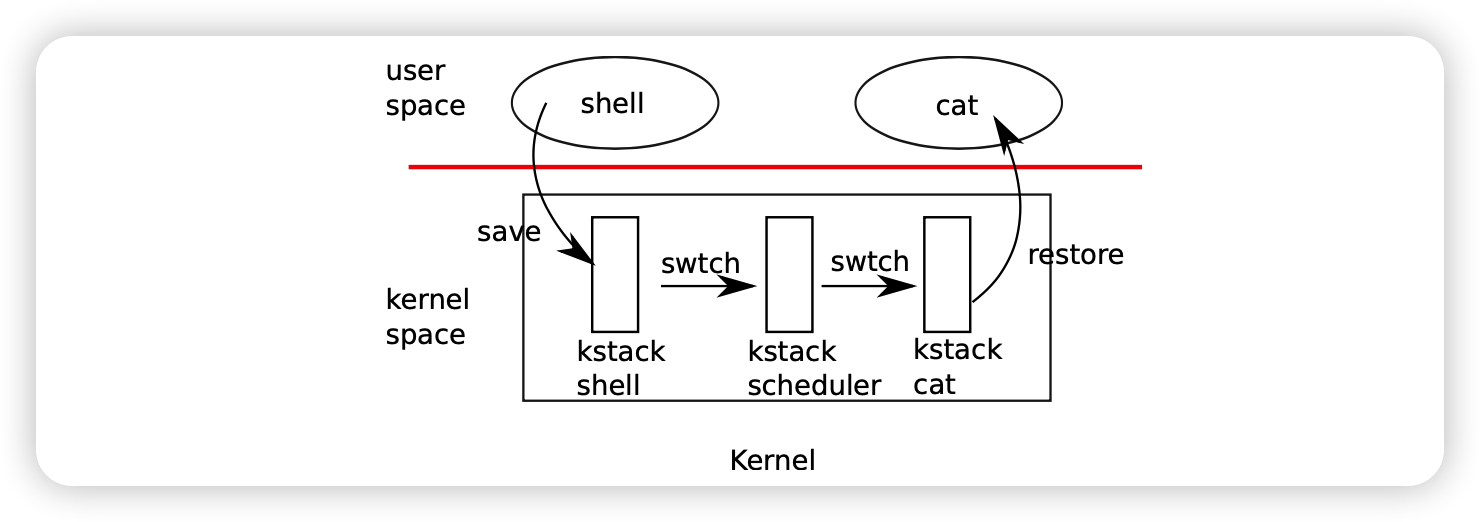
\includegraphics[width=0.8\textwidth]{../imgs/f7-1.png}
    \caption{从一个用户进程切换到另一个。在这个例子中,xv6运行在一个CPU上(因此只有一个调度器线程)。}
    \label{f7-1}
\end{figure}

从一个线程切换到另一个涉及到保存旧线程的CPU寄存器和恢复新线程之前保存的寄存器。
栈指针和程序计数器需要保存和恢复意味着CPU需要切换栈和正在执行的代码。

函数\texttt{swtch}进行内核线程切换时的保存和恢复操作。
\texttt{swtch}并不考虑线程,它只是保存和切换32个RISC-V寄存器,这些寄存器被称为\emph{上下文(context)}。
当进程需要放弃CPU时,进程的内核线程会调用\texttt{swtch}保存它自己的上下文并返回到调度器的上下文。
每个上下文都被存储在一个\texttt{struct context}\href{https://github.com/mit-pdos/xv6-riscv/blob/risc/kernel/proc.h#L2}{(kernel/proc.h:2)}中,这个结构体本身也被包含在进程的\texttt{struct proc}和CPU的\texttt{struct cpu}中。
\texttt{swtch}有两个参数:\texttt{struct context *old}和\texttt{struct context *new}。
它把当前的寄存器保存在\texttt{old}中,从\texttt{new}中获取值加载到寄存器里,然后返回。

让我们跟随\texttt{swtch}进入到调度器中。
我们在\autoref{ch04}中看到过有一种情况下中断的最后一步是\texttt{usertrap}调用\texttt{yield}。
\texttt{yield}再反过来调用\texttt{sched},这个函数会调用\texttt{swtch}来把当前的上下文保存在\texttt{p->context}中,然后切换到保存在\texttt{cpu->context}中的调度器的上下文\href{https://github.com/mit-pdos/xv6-riscv/blob/risc/kernel/proc.c#L497}{(kernel/proc.c:497)}。

\texttt{swtch}\href{https://github.com/mit-pdos/xv6-riscv/blob/risc/kernel/swtch.S#L3}{(kernel/swtch.S:3)}只保存被调者负责保存的寄存器,C编译器在调用者中生成代码来把调用者负责保存的寄存器保存到栈上。
\texttt{swtch}知道\texttt{struct context}中每个寄存器字段的便宜量。
它并不保存程序计数器,而是保存\texttt{ra}寄存器,它保存了\texttt{swtch}结束时应该返回的地址。
现在\texttt{swtch}要根据新的上下文恢复寄存器,新的上下文是新线程之前调用\texttt{swtch}时保存的寄存器。
当\texttt{swtch}返回时,它会返回到恢复的\texttt{ra}寄存器指向的地址,即新线程之前调用\texttt{swtch}时的返回地址。
另外,它会返回到新线程的栈,因为\texttt{sp}寄存器也会被恢复。

在我们的例子中,\texttt{sched}调用\texttt{swtch}来切换到每个CPU的调度器上下文\texttt{cpu->context}。
这个上下文是\texttt{scheduler}上一次调用\texttt{swtch}\href{https://github.com/mit-pdos/xv6-riscv/blob/risc/kernel/proc.c#L463}{(kernel/proc.c:463)}切换到现在正要放弃CPU的进程的时候保存下来的。
当我们正在追踪的\texttt{swtch}返回时,它会返回到\texttt{scheduler}而不是\texttt{sched},并且栈指针现在指向当前CPU的调度器栈。

\section{代码:调度}
上一节介绍了\texttt{swtch}的底层细节,现在让我们看看如何使用\texttt{swtch}从一个进程的内核线程经过调度器到达另一个进程。
调度器是每个CPU的特殊线程,这个线程运行\texttt{scheduler}函数。
这个函数负责选择接下来运行哪个进程。
一个想要放弃CPU的进程必须获取它自己的进程锁\texttt{p->lock},释放它持有的其他所有锁,更新它的状态(\texttt{p->state}),然后调用\texttt{sched}。
你可以在\texttt{yield}\href{https://github.com/mit-pdos/xv6-riscv/blob/risc/kernel/proc.c#L503}{(kernel/proc.c:503)}、\texttt{sleep}、\texttt{exit}中看到这个过程。
\texttt{sched}再次检查这些要求中的一些\href{https://github.com/mit-pdos/xv6-riscv/blob/risc/kernel/proc.c#L487-L492}{(kernel/proc.c:487-492)}然后检查一个隐式条件:因为有一个锁被持有来,所以中断应该被禁用了。
最后,\texttt{sched}调用\texttt{swtch}把当前的上下文保存在\texttt{p->context}中,然后切换到\texttt{cpu->context}中的调度器上下文中。
\texttt{swtch}在调度器的栈中返回,就好像\texttt{scheduler}的\texttt{swtch}返回了一样\href{https://github.com/mit-pdos/xv6-riscv/blob/risc/kernel/proc.c#L463}{(kernel/proc.c:463)}。
然后调度器继续它的\texttt{for}循环,寻找下一个要运行的进程,切换到它,然后重复这个过程。

我们刚才看到xv6在调用\texttt{swtch}的整个过程中持有着\texttt{p->lock}:\texttt{swtch}的调用者必须已经持有了这个锁,然后锁的控制权被传递到切换到的新代码中。
这种转换很不寻常,通常情况下获取锁的线程也应该负责释放锁,这样更容易确保正确性。
但对于上下文来说,打破这个惯例是必须的,因为\texttt{p->lock}负责保护进程的\texttt{state}和\texttt{context}字段上的不变量,但是这些不变量在执行\texttt{swtch}期间并不成立。
一个可能出现的问题是如果在执行\texttt{swtch}期间没有持有\texttt{p->lock},另一个CPU可能会在\texttt{yield}把这个进程的状态设置为\texttt{RUNNABLE}之后但在\texttt{swtch}让它停止使用自己的内核栈之前决定运行它。
结果会是两个CPU在同一个栈上运行,这将导致错误。

内核线程唯一放弃CPU的地方就是\texttt{sched}里,并且它总是切换到\texttt{scheduler}里的同一个地方,(几乎)总是之前调用\texttt{sched}切换到某个内核线程的那个地方。
因此,如果打印出xv6切换线程的行号,将会观测到下面的一个简单模式:\href{https://github.com/mit-pdos/xv6-riscv/blob/risc/kernel/proc.c#L463}{(kernel/proc.c:463)}、\href{https://github.com/mit-pdos/xv6-riscv/blob/risc/kernel/proc.c#L497}{(kernel/proc.c:497)}、\href{https://github.com/mit-pdos/xv6-riscv/blob/risc/kernel/proc.c#L463}{(kernel/proc.c:463)}、\href{https://github.com/mit-pdos/xv6-riscv/blob/risc/kernel/proc.c#L497}{(kernel/proc.c:497)}等等。
主动通过线程切换互相转移控制权的过程有时也被称为\emph{协程(coroutine)},
在这个例子中,\texttt{sched}和\texttt{scheduler}就是彼此的协程。

有一种情况下调度器对\texttt{swtch}的调用并不会以\texttt{sched}结束。
\texttt{allocproc}把新进程的上下文\texttt{ra}寄存器设置为\texttt{forkret}\href{https://github.com/mit-pdos/xv6-riscv/blob/risc/kernel/proc.c#L515}{(kernel/proc.c:515)},因此它的第一个\texttt{swtch}会“返回”到那个函数的起始位置。
\texttt{forkret}的存在是为了释放\texttt{p->lock};否则,由于新进程需要像从\texttt{fork}返回一样返回用户空间,它可能会从\texttt{usertrapret}开始。

\texttt{scheduler}\href{https://github.com/mit-pdos/xv6-riscv/blob/risc/kernel/proc.c#L445}{(kernel/proc.c:445)}运行一个循环:找到一个要运行的进程、运行它直到它让出CPU,然后重复。
调度器循环遍历进程表寻找一个可以运行的进程,即\texttt{p->state == RUNNABLE}的进程。
一旦它找到了一个进程,它会设置每个CPU用于表示当前进程的变量\texttt{c->proc},然后把进程标记为\texttt{RUNNING},并调用\texttt{swtch}开始运行它\href{https://github.com/mit-pdos/xv6-riscv/blob/risc/kernel/proc.c#L458-L463}{(kernel/proc.c:458-463)}。

考虑调度器代码结构的一种思路是它对每个进程强迫执行一组不变量,并在不变量不成立时持有\texttt{p->lock}。
一个不变量是如果一个进程是\texttt{RUNNING},那么时钟中断的\texttt{yield}必须能安全地切换离开这个进程;这意味着CPU寄存器必须持有这个进程的寄存器的值(即,\texttt{swtch}还没有把它们移动到\texttt{context}中),并且\texttt{c->proc}必须指向这个进程。
另一个不变量是如果一个进程是\texttt{RUNNABLE},一个空闲CPU的\texttt{scheduler}运行它必须是安全的;这意味着\texttt{p->context}必须持有这个进程的寄存器(即,它们并不在真正的寄存器中),并且没有CPU正在这个进程的内核栈上执行,并且没有CPU的\texttt{c->proc}指向这个进程。
当\texttt{p->lock}被持有时这些条件通常并不成立。

xv6之所以经常在一个线程中获取\texttt{p->lock}而在另一个线程中释放它,是为了维护上述的不变量,例如在\texttt{yield}中获取锁并在\texttt{scheduler}中释放它。
一旦\texttt{yield}开始修改一个正在运行的进程的状态把它改为\texttt{RUNNABLE},锁必须被持有直到不变量恢复:最早的正确释放锁的地方是在\texttt{scheduler}(在它自己的栈上运行)清除\texttt{c->proc}之后。
类似地,一旦\texttt{scheduler}开始把一个\texttt{RUNNABLE}进程转换为\texttt{RUNNING},锁在内核线程完全开始运行(\texttt{swtch}之后,例如\texttt{yield}中)之前不能被释放。
